\documentclass[../main/IoT.tex]{subfiles}
\begin{document}
\section{Introduction and Background}\label{intro}
\subsection{Self-governing, decentralized, extensible IoT, connected to a shared, variable power supply. Each thing is an object.}
A lot of effort is invested when comes to managing and distributing resources to large, almost implied distributed systems. A common resource of this type is the power resource; powering all kinds of ``things'' around us, such as households appliances (fridge, computer, toaster etc.), heating systems (e.g. of the house, of the office), etc. The Internet of Things (IoT) is a term to describe such networked ``things'', objects not traditionally thought of as computers (e.g. cars, household appliances), which may nonetheless be connected using Internet protocols and technologies (TCP/IP, etc.). Assuming such a network of objects, connected to a shared power supply, in this paper we are creating a framework for a Self-Governing, Decentralized, Extensible, Non-Preemptive IoT, where objects communicate and cooperate together to achieve system efficiency (in terms of power consumption).

The naive approach to the IoT would use a central controller or master node of some sort to oversee the activities of all objects of the system, and make decisions on behalf of the objects (e.g. decide when the toaster should be powered). However, the approach has got clear limitations and drawbacks, not the least being scalability. We are talking about an extensible large system, where new objects can join the system at any point. One other issue may be the reliability of the system. If \emph{the single point of failure (SPOF)} exists, the entire system would stop working, and all objects of the system would fail to get powered.

A decentralized approach however, would better fit the needs of such IoT, overtaking the limitations mentioned above. All objects of the system would required to have a controller of some kind, which provides them with computing capabilities. This would make them capable of making own decisions, therefore let us call them self-governing objects. Liu and Zhou \cite{IoT6150221} describes such property as ``autonomy Feature'' of objects, where objects have the ability to reason, negotiate, understand, adapt and learn from other objects or environments. Such an Internet of Things with self-governing ``things'' would not require a central controller, and addition or removal of ``things'' would be far easier.

\subsection{Prioritized objects, cooperating and creating individual views of the system}
We described an IoT system where objects are interconnected, and in the same time connected to a power supply. Each object of the system consumes an amount of power resource, that can be different from object to object (e.g. a toast will consume less power than a washing machine). We assume this amount to be constant for each object, that means each object consumes a fixed amount of power or none, and this amount cannot change in time.

The power supply is something that supplies the system with power resource. In the real world, if we think of power suppliers, they might provide a variable amount of power budget, that means at different times there is different power resource available (e.g. thinking of a wind turbine, the provided power resource would be dependant on how much wind there is). Therefore, we assume the power resource to be variable in time and dependent on some external factors. We will also assume that there is only one power supply in the IoT system.

The total demand of system at any one time (regardless of resource), as described by Rao~\cite{rao2011foundation}, is the sum of all resource demands for all processes in a system. In our case, the total demand of power resource is the sum of all power demands of all objects in the system. One question is, what happens if the total demand of the system exceeds the power resource provided by the power supply. The answer is we cannot satisfy all objects with power. We are assuming that we cannot partially fulfill an object with power. It is either powered, therefore it consumes the fixed amount of power demand it requested, or not powered and consumes nothing. Rao~\cite{rao2011foundation} describes that in practice, distributed processes (objects in our case) drawing some sort of resource (power resource in our case), are distinguished from one another in terms of some sort of priorities. This is because some objects are more important than others in terms of their functions and utilities, and if the power supply cannot satisfy all the objects, priority will distinguish between which objects should be powered with the available power resource. Following the presented approach, objects with higher priority will be provided with power resource first (See Figure \ref{fig1})
\begin{figure}[h]
  \centering
  % Requires \usepackage{graphicx}
  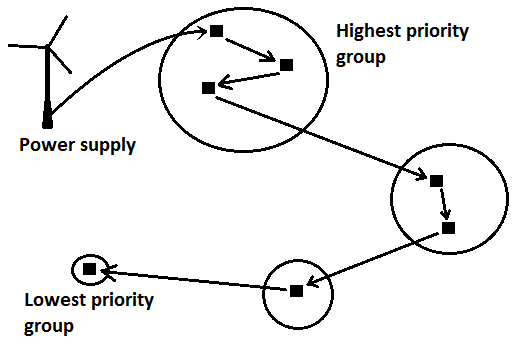
\includegraphics[width=80mm]{../figs/model.png}\\
  \caption{The flow of powering the system after priorities.}\label{fig1}
\end{figure}

Not having a central controller, all objects of the system need to decide when it is a suitable time for them to get powered. Therefore, they need to have a general overview of their position in the system in terms of their priority compared to other objects priorities and their power demand compared with other objects power demand. They achieve this by communicating and informing other objects about their details, while receiving information from all the other objects.

All the objects in our IoT framework are connected, networked between them such that any object in the system can communicate - send or receive a message - with/from any other object in the system. Prasad and Kumar \cite{prasad2012energy} describes this particular aspect of IoT as the advance version of Machine to Machine communication, where objects are exchanging information between them without a human intervention. When sending a message, we will later describe two types of destinations: one to one message (where the message is sent from one object to another specific object), and message broadcasting (where messages are broadcasted/flooded over all other objects in the system - see Algorithm \ref{flood} in the further section). For simplicity of the model, we make abstraction of how objects are connected.

We are describing a system with non-preemptive power policy; meaning that there is no partial fulfillment. When an object was allocated power resource, it is not interrupted until it has finished its demands, or there is a change in the available power resources. In other words, if a new object with high priority joins the system at some point and a low priority object has been allocated with power, the new object has to wait until the low priority object is leaving the system, or more power is provided by the power supply. In the same time, there should be no dependencies between objects except priorities. That is when the available power resource exceeds the total demand of the system, all objects of the system shall be powered, and no object shall wait for a different object to finish its demands or leave the system.

\subsection{Background and Related Work}

In this subsection we will discuss the related work and background information close to our focus. 

Higgins et al. \cite{higgins2011distributed} discussed ``a pathway'' to flexible power system automation. He proposed a new approach, based on ``distributed intelligence'' rather than ``traditional centralized control'', the system benefiting on many levels. We further considered Higgins approach by creating a decentralized distributed model of IoT, where power resource consumers can join and leave the system, and in the same time, they adapt automatically when needed (either a change in power or when consumers are joining or leaving the system).

One aspect of the IoT, Zorzi et al \cite{zorzi2010today} points out, is a first time opportunity to interact with the surrounding environments and to exchange information that previously was not available. He points out a series of issues when comes to IoT paradigm including connectivity, scalability, self-management capability, and energy management. In this paper we answer some of the issues addressed by Zorzi, and create a connected, extensible IoT, where objects are ``smart things'' with self-governing capabilities to apply it within energy management problem.

Niyato et al. \cite{niyato2011machine} presents a framework

In this section we introduced the topic and presented an overview of our interest. The following section is to describe the framework of IoT by creating a model of such system, developing some algorithms for the distributed IoT, and at the end presenting and developing some profs of correctness of our work.

\end{document} 